\section{Images}
\subsection{light}
\[
c = \lambda \cdot f \quad c = \text{speed of light} = 3 \cdot 10^8 \text{m/s}
\]
Relevant ranges for \(\lambda\) in image processing:
\begin{itemize}
    \item \textbf{UV:} 100 nm - 380 nm: UV-A (315-380 nm)
    \item \textbf{Visible light:} 380 nm (green) - 700 nm (red)
    \item \textbf{IR:} 780 nm - 1 mm: IR-A , IR-B 
\end{itemize}
\begin{figure}
    \centering
    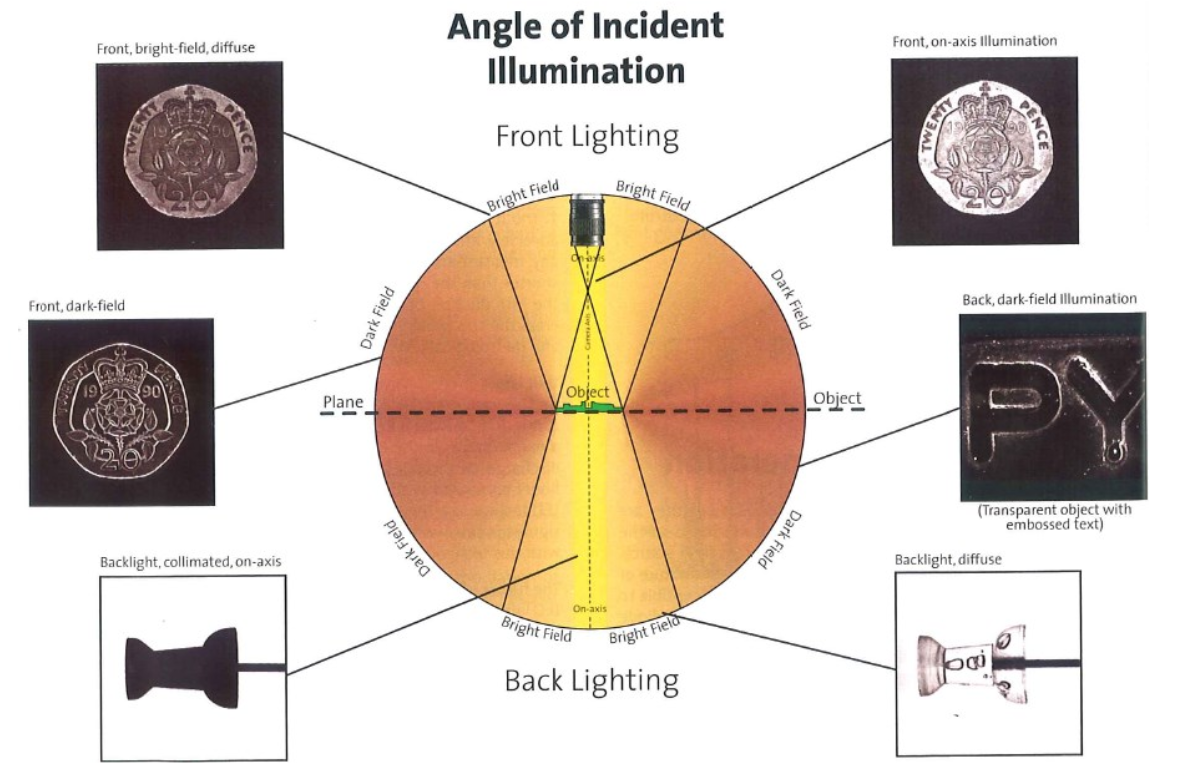
\includegraphics[width=0.8\columnwidth]{Images/02/Illumination.png}
    \caption{Angle of Incidence}
    \label{fig:02_Illumination}
\end{figure}
\subsection{Image Formation: Optics and Cameras}
\begin{itemize}
    \item Field of View (FoV): Area covered by the camera frame
    \item Working Distance (WD): Distance between camera focal point and object
    \item Resolution: The minimum feature size of the object that the imaging system can distinguish.
    \item Depth of Field (DOF): The range of distance photograph where objects appear sharp and in focus.
    \item Sensor Size: The size of a camera sensor's active area
    \item PMAG: The Primary Magnification of the lens is the ratio between the sensor size and the FOV.
\end{itemize}

\subsection{2D imahes as a discrete function}
Image Size / Sampling:
\begin{itemize}
    \item  M (rows) * N (columns) pixels (picture
    elements)
    \item Spatial resolution:
    \begin{itemize}
        \item size in the real world (e.g. dpi, lpi, pixel/m, …)
    \end{itemize}
    \item Coordinate system:
    \begin{itemize}
        \item origin in upper left corner,
        \item x-axis downwards, y-axis to the right!
    \end{itemize}
\end{itemize}
Quantization: Number of intensity values:
\begin{itemize}
    \item e.g 8 bit (256 values)
    \item Int:{0(black), 255(white)} or Double:{0.0(black), 1.0(white)}
\end{itemize}